\documentclass[10pt]{article}

\usepackage{amsmath,amssymb,amsthm}

\usepackage{blindtext}
\usepackage[a4paper, total={6in, 8in}]{geometry}


% Theorem and color box settings
\usepackage{tcolorbox}
\usepackage{tikz}
\tcbuselibrary{theorems}

\usepackage{xcolor}      % For color definitions
\definecolor{custom_green}{HTML}{a3be8c}
\definecolor{custom_red}{HTML}{bf616a}

% Theorem box
\newtcolorbox{theorembox}[1][]{
  title={#1},
  fonttitle=\bfseries,
  colback=custom_green!30!white,
  colframe=custom_green,
  coltitle=black,
  boxrule=0.5pt,
  arc=4pt,
  outer arc=4pt,
}

\newtcolorbox{examplebox}[1][]{
  title=\textbf{Example:} {#1},
  fonttitle=\bfseries,
  colback=custom_red!20!white,
  colframe=custom_red,
  coltitle=white,
  boxrule=0.5pt,
  arc=4pt,
  outer arc=4pt,
}

\begin{document}
\section{Complex Analysis}
    \subsection{Mobius Transforms}
        \textbf{Recall:} The complex plane $\mathbb{C}$ can be throught as points $(x,y) \in \mathbb{R}^2$, but we usually label a point as $z = x+iy$.
        We can extend $\mathbb{C}$ by adding a point at infinity, the resulting set is called the \textbf{Riemann Sphere} $\tilde{\mathbb{C}}$.
        Visually, we can imaigine wrapping the complex plane onto the surface of a sphere, where $\infty$ is the north pole of the sphere. \\[2ex]
        \noindent Now, letting $a,b,c,d$ be complex numbers (i.e. $ a = x_a + iy_a$), we define a Mobius Transform as a function $T:\tilde{\mathbb{C}} \to \tilde{\mathbb{C}}:$
        $$T(z) = \frac{az + b}{cz +d}$$
        where $ad -bc \neq 0$ (that is the determinant $\neq$ 0 $\rightarrow$ matrix is invertible). \\
        These functions occur on the Riemann Sphere, because we need to define that happens when $cz + d = 0$ and when $z = \infty$:
    
        $$\text{If} \;c \neq 0: \quad T(\infty) = \frac{a}{c} \quad \text{and} \quad T\left(-\frac{d}{c}\right) = \infty$$
        $$\text{If} \;c = 0: \quad T(z) = \frac{az + b}{d}\quad \text{and} \quad T(\infty) = \infty$$ 
        
        \noindent Mobius transforms can be  uniquely determined by its action on three distinct points. For example, we'll find a mobius transform that maps three points $\{z_1, z_2, z_3\}$ to $\{1,0,\infty\}$ \\[2ex]
        1. We want $T(z_2) = 0 : az_2 + b = 0 \Rightarrow b= -az_2$ , then $T(z)$ becomes: 
        $$T(z) = \frac{az + b}{cz + d} = \frac{az -az_2}{cz+d} = \frac{a(z-z_2)}{cz + d}$$
        2. We want $T(z_3) = \infty : cz_3 + d = 0 \Rightarrow d = -cz_3$, then $T(z)$ becomes:
        $$T(z) = \frac{a(z - z_2)}{c(z - z_3)}$$
        3. We want $T(z_1) = 1$, then $T(z_1)$ becomes:
        $$T(z_1) = \frac{a(z_1 - z_2)}{c(z_1 - z_3)} = 1 \Rightarrow \frac{a}{c} = \frac{z_1 - z_3}{z_1 - z_2}$$
        Finally, we see that $T(z)$ is:
        $$T(z) = \frac{z_1 - z_3}{z_1 - z_2}\cdot \frac{z - z_2}{z - z_3} $$
        We can now solve problems, such as : Find the Mobius Transform that maps the 3 points $z_1 = -i, z_2 = -1, z_3 = 1$ to $1,0,\infty$ 
        $$T(z) = \frac{-1 -1}{i + 1} \cdot \frac{z + 1}{z-1} = (-i)\frac{z+1}{z-1} = \frac{-iz -i}{z-1}$$
        
        \pagebreak 

        \subsubsection{Matrix Representation of Mobius Transforms}
        We associate a $2 \times 2$ matrix $M$ to a Mobius Transform $T(z)$:
        $$T(z) = \frac{az + b}{cz + d} \longleftrightarrow M  = \begin{bmatrix}a & b \\c & d\end{bmatrix}$$
        \indent \emph{Note that:} $kM \longleftrightarrow T(z)$ for any $k \in \mathbb{C}, k \neq 0$. \\[2ex]
        We can also define the \textbf{inverse map} $T^{-1}$ as the Mobius transform:
        $$T^{-1} \longleftrightarrow \begin{bmatrix}d & -b \\ -c & a\end{bmatrix}$$
        We can also define the \textbf{composition} of two Mobius Transforms, if $T_1(z) = \frac{az + b}{cz + d}$ with matrix $M$ and $T_2(z) = \frac{ez + f}{gz + g}$ with matrix $M_2$, then:
        $$
        T \circ T_2 \longleftrightarrow  
        \begin{bmatrix}
            a & b \\ c & d
        \end{bmatrix}
        \cdot
        \begin{bmatrix}
            e & f \\ g & h
        \end{bmatrix}
        =
        \begin{bmatrix}
            ae + bg & af + bh \\ ce + dg & cf + dh
        \end{bmatrix}
        $$
        Putting it all together, we can map any three points to any other three point: 
        \begin{theorembox}[Three-Point Theorem for Möbius Transformations]
            If $T \longleftrightarrow M : (z_1, z_2, z_3) \mapsto (1,0,\infty)$ and if $T_2 \longleftrightarrow M_2: (z'_1, z'_2, z'_3) \mapsto (1,0,\infty)$ then:
            $$T^{-1} \circ T_2 \longleftrightarrow M^{-1} \cdot: (z_1, z_2, z_3) f\mapsto (z'_1, z'_2, z'3) $$
            This can be visualized like so:
            \begin{center}
                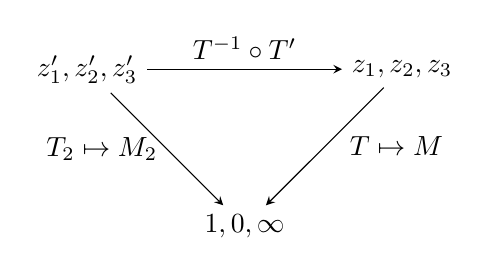
\begin{tikzpicture}[>=stealth, auto]
                    \node (A) at (0,2) {$z'_1, z'_2, z'_3$};
                    \node (B) at (4, 2) {$z_1, z_2, z_3$};
                    \node (C) at (2,0) {$1, 0, \infty$};

                    \draw[->] (A) -- (B) node[above, midway] {$T^{-1} \circ T'$};
                    \draw[->] (A) -- (C) node[left, midway] {$T_2 \mapsto M_2$};
                    \draw[->] (B) -- (C) node[right, midway] {$\;\;T \mapsto M$};
                \end{tikzpicture}
            \end{center}
            Note that, $M, M_2$ and $T^{-1}\circ T_2$ have matrices: Three-Point Theorem for Möbius Transformations
            \footnotesize$$M = \begin{bmatrix} a&b \\ c &d \end{bmatrix}, \quad M_2 = \begin{bmatrix} e&f \\ g &g \end{bmatrix}, \quad T^{-1} \circ T_2 =  \begin{bmatrix} d&-b \\ -c &a \end{bmatrix} \cdot \begin{bmatrix}e & f \\ g & h\end{bmatrix}$$
        \end{theorembox}
        
        \begin{examplebox}[Find a Mobius transformation, $T:  (0,-i,-1) \mapsto (i, 1, 0)$]
            If we can find a map $T_1 : (0, -i, 1) \mapsto (1, 0, \infty)$ and a map \\
             $T_2 : (1, -i, -1) \mapsto (i, 1, 0)$. Then, by the Theorem above, we can find a $T$ such that: $T:(0, -i, -1) \mapsto (i, 1,0)$ 
            Recall, we define a general transform $T$, that takes 3 points $(z_1, z_2, z_3) \mapsto (1, 0, \infty)$
            $$T(z) = \frac{z_1 - z_3}{z_1 - z_2} \cdot \frac{z - z_2}{z - z_3} $$
            \noindent
            \begin{minipage}{0.45\textwidth}
                $T_1$ becomes:
            \begin{align*}
                T_1(z) &= \frac{0 +1}{0+i} \cdot \frac{z+i}{z+1} \\
                &= \frac{1}{i}\cdot \frac{z+i}{z+1} \\
                &= \frac{z+1}{iz + i} \\
                &\Rightarrow \begin{bmatrix}1 & i \\ i & i \end{bmatrix}
            \end{align*}
            \end{minipage}
            \begin{minipage}{0.45\textwidth}
                $T_2$ becomes:
                \begin{align*}
                    T_2(z) &= \frac{i-0}{i-1} \cdot \frac{z-1}{z-0} \\ 
                    &= \frac{i}{i-1} \cdot \frac{z-1}{z} \\
                    &= \frac{iz - i}{(i-1)z } \\
                    &\Rightarrow \begin{bmatrix}i & -i \\ i-1 & 1 \end{bmatrix}
                \end{align*}
            \end{minipage}
            \hfill \\[2ex]
            Thus, $T$ is:
            $$T =T^{-1}_2 \circ T_1 \leftrightarrow \begin{bmatrix}1 & i \\ i & i\end{bmatrix} \cdot \begin{bmatrix} i & -i \\ i-1 & 0 \end{bmatrix}^{-1}$$
            \scriptsize$$
            = \begin{bmatrix}1 & i \\ i & i\end{bmatrix} \cdot \begin{bmatrix}0 & i \\ 1 & i-1\end{bmatrix} 
            = \begin{bmatrix}1 & i \\ i & i\end{bmatrix} \cdot \begin{bmatrix}i & -i \\ i-1 & 1\end{bmatrix} 
            = \begin{bmatrix} 0(1) + (i)(i) & (0)(i) + (i)(i) \\ (1-i)(1)+ (i)(i) & (1-i)(i) + (i)(i)\end{bmatrix} 
            = \begin{bmatrix} i^2 & i^2 \\ -i & i\end{bmatrix}
            $$
            \normalsize$$T(z)  = -\begin{bmatrix}1 & 1 \\ i & -i \end{bmatrix}\longleftrightarrow = -i \frac{z+1}{z-1}$$

        \end{examplebox}
        


    
        \end{document}
